\documentclass{article}
\usepackage[a4paper, total={6in, 9in}]{geometry}
\usepackage{graphicx}
\usepackage{xcolor}
\usepackage{listings}
\definecolor{vgreen}{RGB}{104,180,104}
\definecolor{vblue}{RGB}{49,49,255}
\lstset{
    language=Verilog,
    % wrap text
    breaklines=true, 
    % line numbers
    numbers=left,
    numberstyle=\tiny\color{black},
    numbersep=10pt,
    % other styling
    basicstyle=\small\ttfamily,
    keywordstyle=\color{vblue},
    identifierstyle=\color{black},
    commentstyle=\color{vgreen},
    tabsize=2
}
\graphicspath{ {images/} }

\title{
    \begin{large}
        ELEC374 - Lab 1
    \end{large}
}
\author{Naod Dereje - 20103501, Thierry Jones - 20108349, Jamie Won - 20113217}

\begin{document}
\maketitle
\cleardoublepage
\tableofcontents
\cleardoublepage

\section{Components}
    The purpose of this lab was to design and simulate a part of the mini SRC datapath. A bus, MDR, ALU, datapath and 16 registers were needed to do so. Verilog was chosen over VHDL as it is better for more complex simulations. The verilog code for each of these components can be found in the Appendices.

    \subsection{Bus}
    The bus was implemented using a 32-to-5 bit encoder. The verilog code for this component can be found in Appendix \ref{Bus}

    \subsection{Memory Data Register (MDR)}
    The memory data register was implemented with a 32 bit multiplexer and flip flop. The code for the flip flop can be found below.
        \lstinputlisting{Modules/dff_32bit.v}
    The code for the multiplexer can be found below.
        \lstinputlisting{Modules/mux21_32bit.v}
    Finally, the code for the MDR itself can be found in Appendix \ref{MDR}

    \subsection{Datapath}
    The datapath module connects all the other modules. There are some internal connections that were made, as well as 16 registers that were created. The code for a single register can be found below.
        \lstinputlisting{Modules/Register.v}
    The verilog code for the datapath can be found in Appendix \ref{Datapath}.

    \subsection{Arithmetic Logic Unit (ALU)}
    The ALU is able to perform addition, subtraction, multiplication, division, not, negation, and, shifting left and right, and rotating left and right. The verilog code for these operations as well as the ALU itself can be found in Appendix \ref{ALU}.

\section{Circuitry Demonstration}

    To demonstrate the success of the ALU, multiple testbenches were created to simulate each operation. Barring the control sequence, the testbenches are all identical to the one found in Appendix \ref{Testbench} The following subsections of the report detail the changes made in the test bench due to the control sequence changing as well as the waveforms generated by each simulation. It should be noted that not all possible waves were added to the images shown. This was due to redundancy - there is no reason to have multiple clock signals, nor registers that aren't used. In order to more accurately show to specific operations that were executed, some changes were made to the testbenches functionality. For AND, OR, SHR, SHL, ROR, ROL, instructions were converted to hexidecimal values to show each four bits as a number representation. This was done since decimal is difficult to read bit patterns from. For the MUL, DIV, ADD, SUB, NEG operations, the values for the high and low bits were read as decimal values to more accurately depict result of arithmetic for a user reading the waveforms.

    \subsection{and R5, R2, R4}
    This instruction demonstrates the ALU's and circuitry. The control sequence for this instruction was provided in the lab manual. The control sequence for this instruction can be found below in Appendix \ref{AND}.
    
    \begin{figure}[h!]
        \begin{center}
            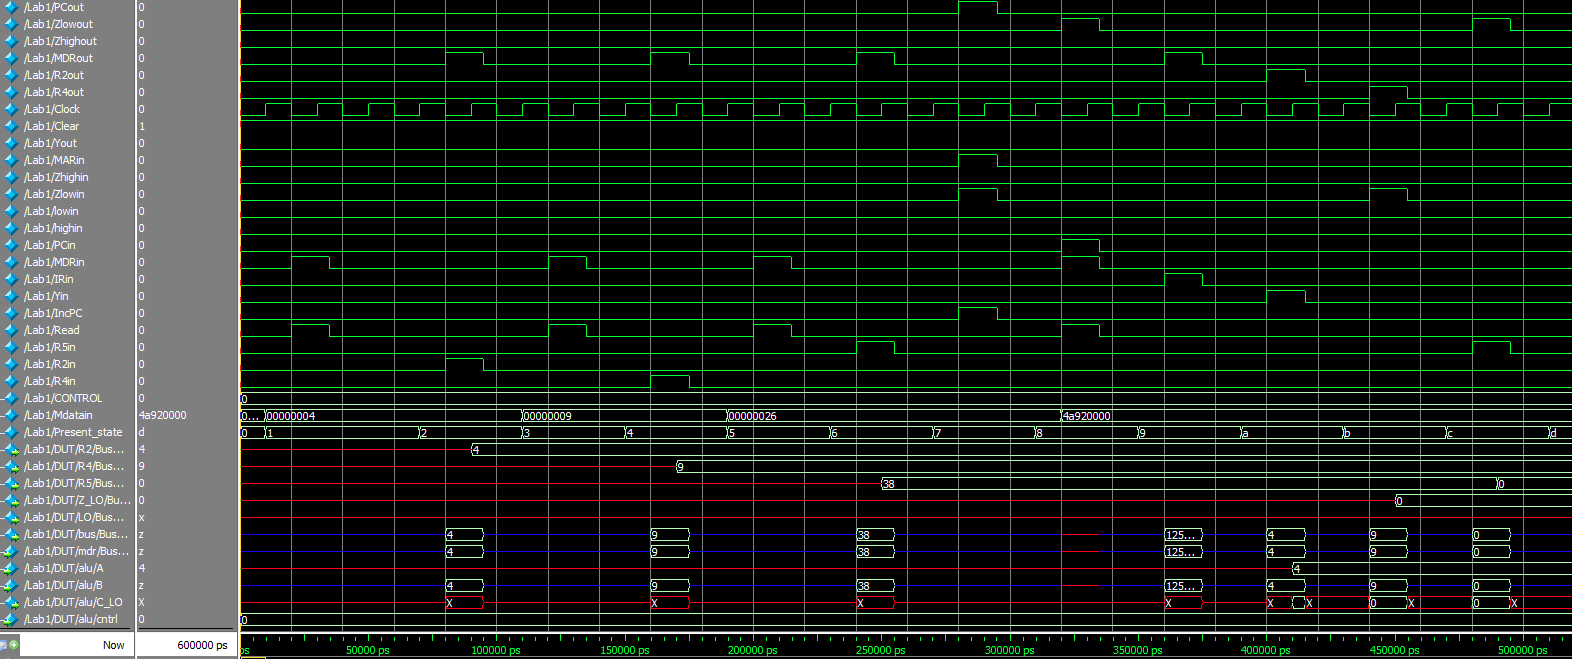
\includegraphics[width=15cm]{AND_FINAL.png}
            \caption{A screenshot of the simulated waveforms for the and R5, R2, R4 instruction}
        \end{center}
    \end{figure}

    \subsection{or R5, R2, R4}
     This instruction demonstrates the ALU's or circuitry. The control sequence is the same as AND with 5 stages. Furthermore, the CONTROL signal is changed to that of the or command. The control sequence for this instruction can be found below in Appendix \ref{OR}.
     
    \begin{figure}[h!]
        \begin{center}
            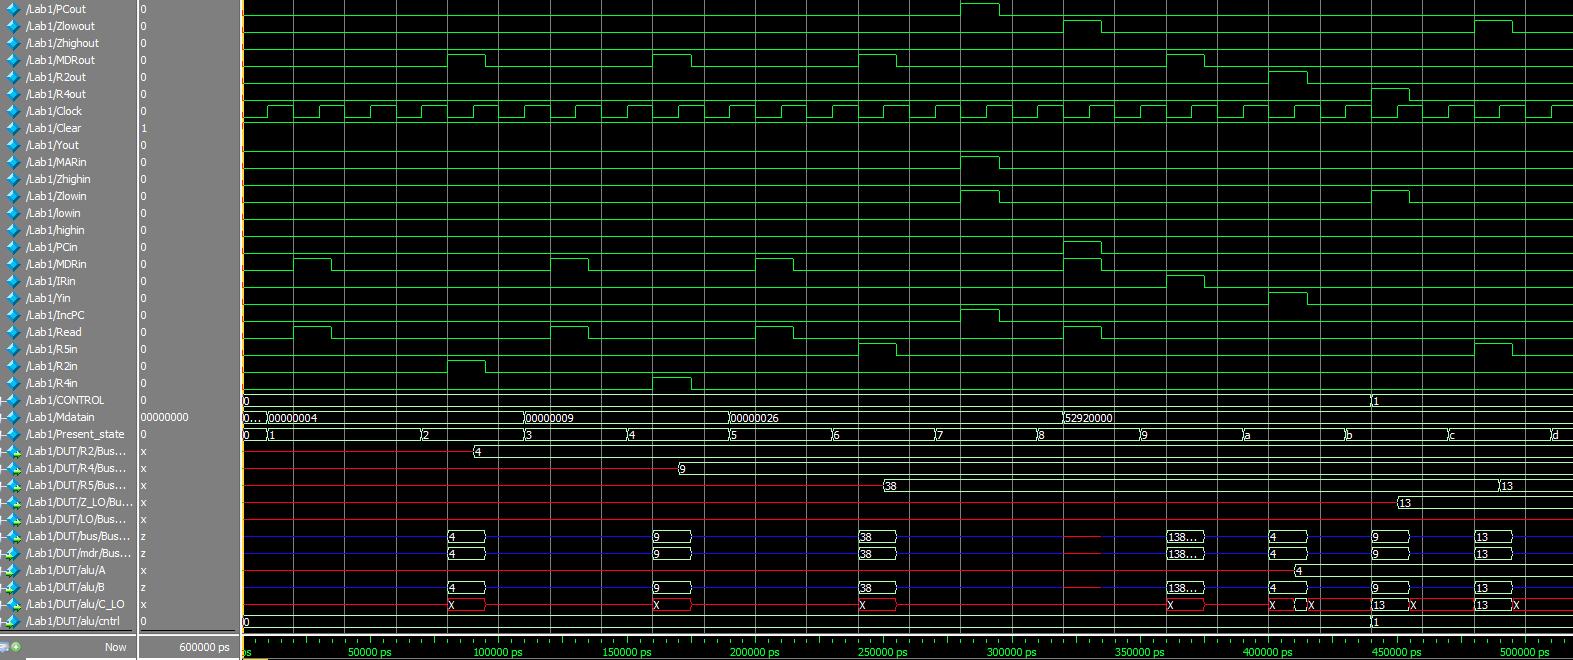
\includegraphics[width=15cm]{OR_FINAL.png}
            \caption{A screenshot of the simulated waveforms for the or R5, R2, R4 instruction}
        \end{center}
    \end{figure}
     
    \subsection{add R5, R2, R4}
     This instruction demonstrates the ALU's add circuitry. The control sequence is the same as or with 5 stages. Furthermore, the CONTROL signal is changed to that of the add command. The control sequence for this instruction can be found below in Appendix \ref{ADD}.
     
    \begin{figure}[h!]
        \begin{center}
            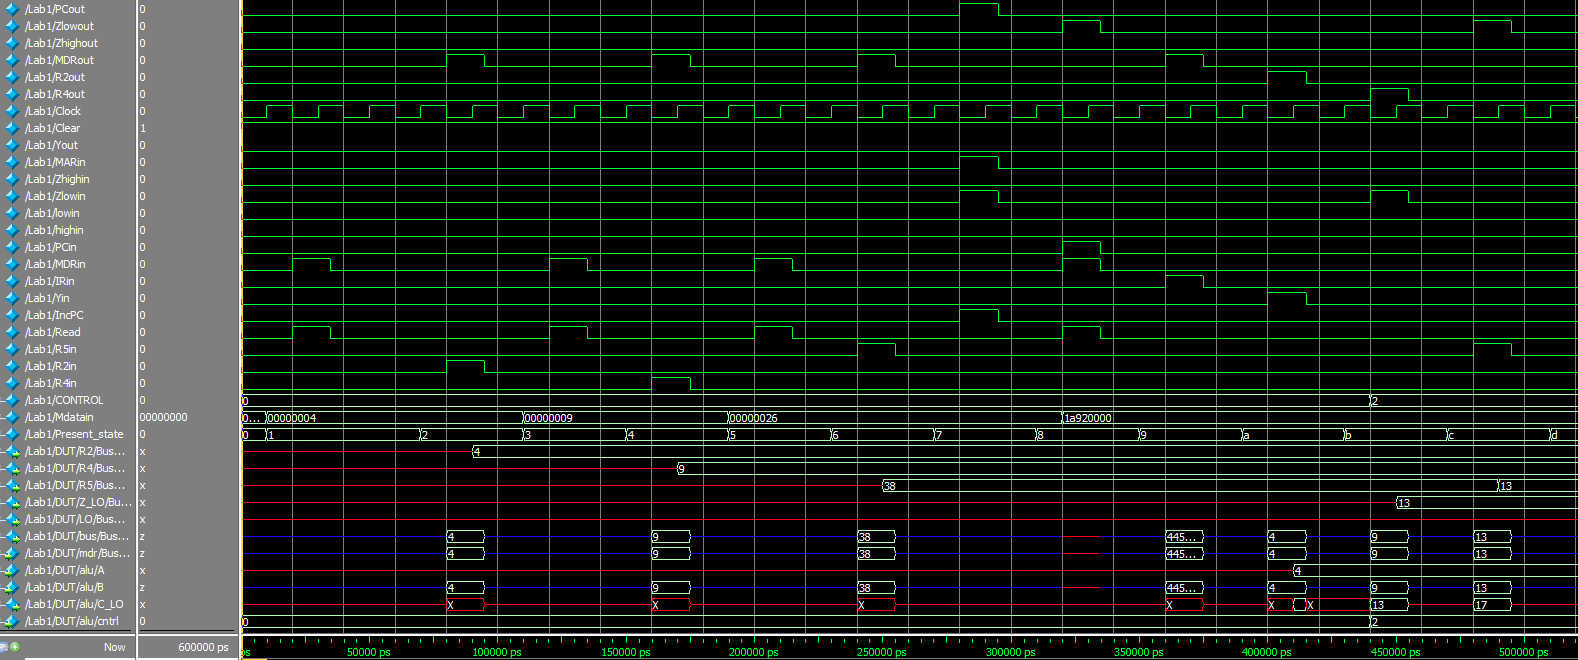
\includegraphics[width=15cm]{ADD_FINAL.png}
            \caption{A screenshot of the simulated waveforms for the add R5, R2, R4 instruction}
        \end{center}
    \end{figure}
     
    \subsection{sub R5, R2, R4}
     This instruction demonstrates the ALU's sub circuitry. The control sequence is the same as add with 5 stages. Furthermore, the CONTROL signal is changed to that of the sub command. The control sequence for this instruction can be found below in Appendix \ref{SUB}.
     
    \begin{figure}[h!]
        \begin{center}
            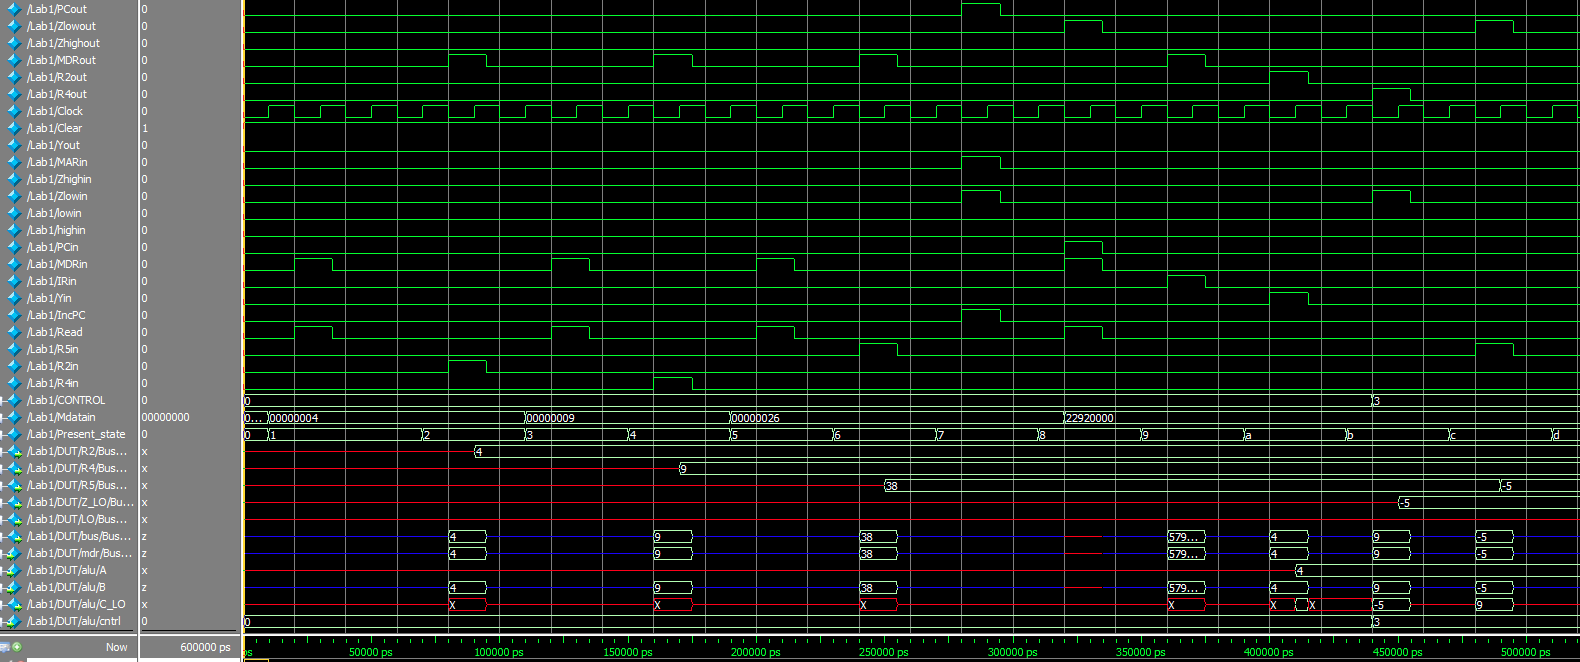
\includegraphics[width=15cm]{SUB_FINAL.png}
            \caption{A screenshot of the simulated waveforms for the sub R5, R2, R4 instruction}
        \end{center}
    \end{figure}
     
    \subsection{mul R2, R4}
    
    The mul instruction control sequence can be found in the mul module code in Appendix \ref{MUL_ALG}, our team used booth's algorithm to generate the multiplication of two numbers in binary form. 
    
    \begin{figure}[h!]
        \begin{center}
            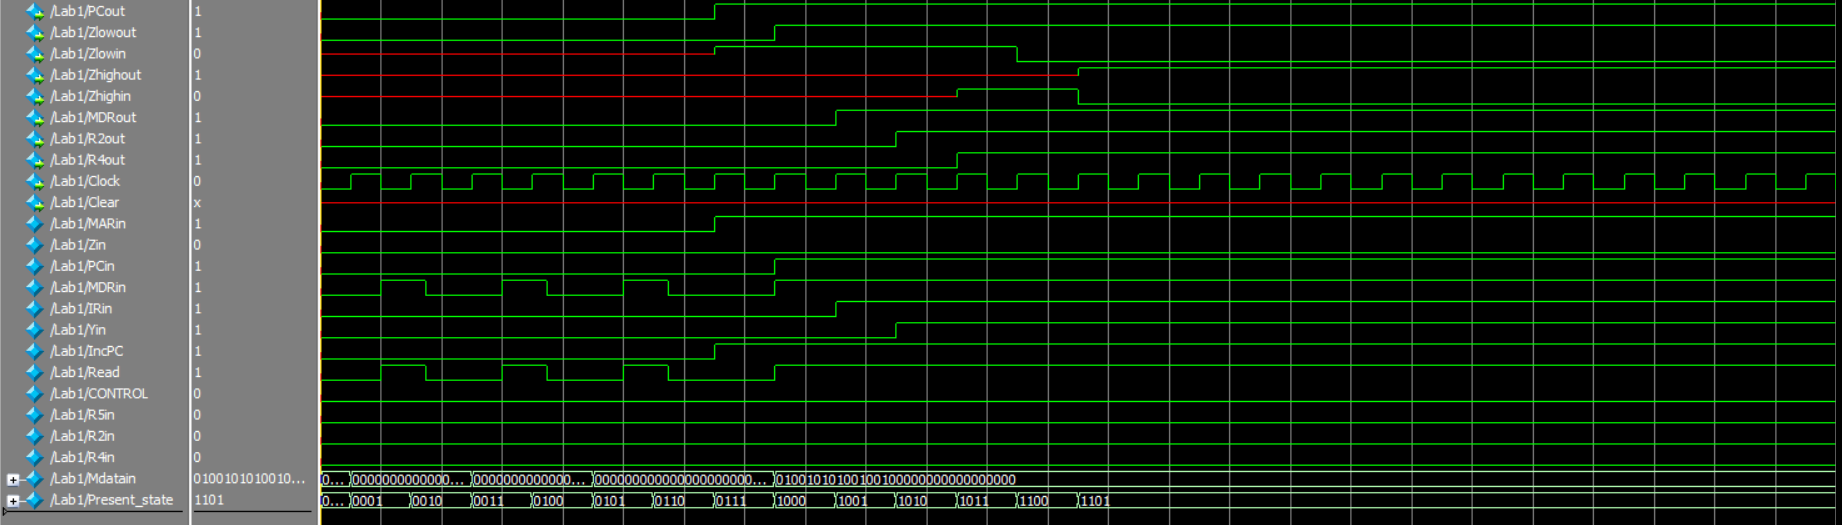
\includegraphics[width=15cm]{mul}
            \caption{A screenshot of the simulated waveforms for the mul R2, R4 instruction}
        \end{center}
    \end{figure}

    \subsection{div R2, R4}
    
    This instruction demonstrates the ALU's division circuitry. This differs from the control sequence in the testbench shown with the addition of a sixth stage, a change in the CONTROL signal to that of the division command and having two 32 bit outputs (Zlowout, Zhighout) as opposed to one. These changes can be found from stages 4-6. The control sequence for this instruction can be found below in Appendix \ref{DIV}. Furthermore, the division was implemented with the algorithm found in Appendix \ref{DIV_ALG}. Furthermore, the quotient is stored in the Z\_LO register and the remainder in Z\_HI. The figures below simulate division with and without remainder.
    
    \begin{figure}[h!]
        \begin{center}
            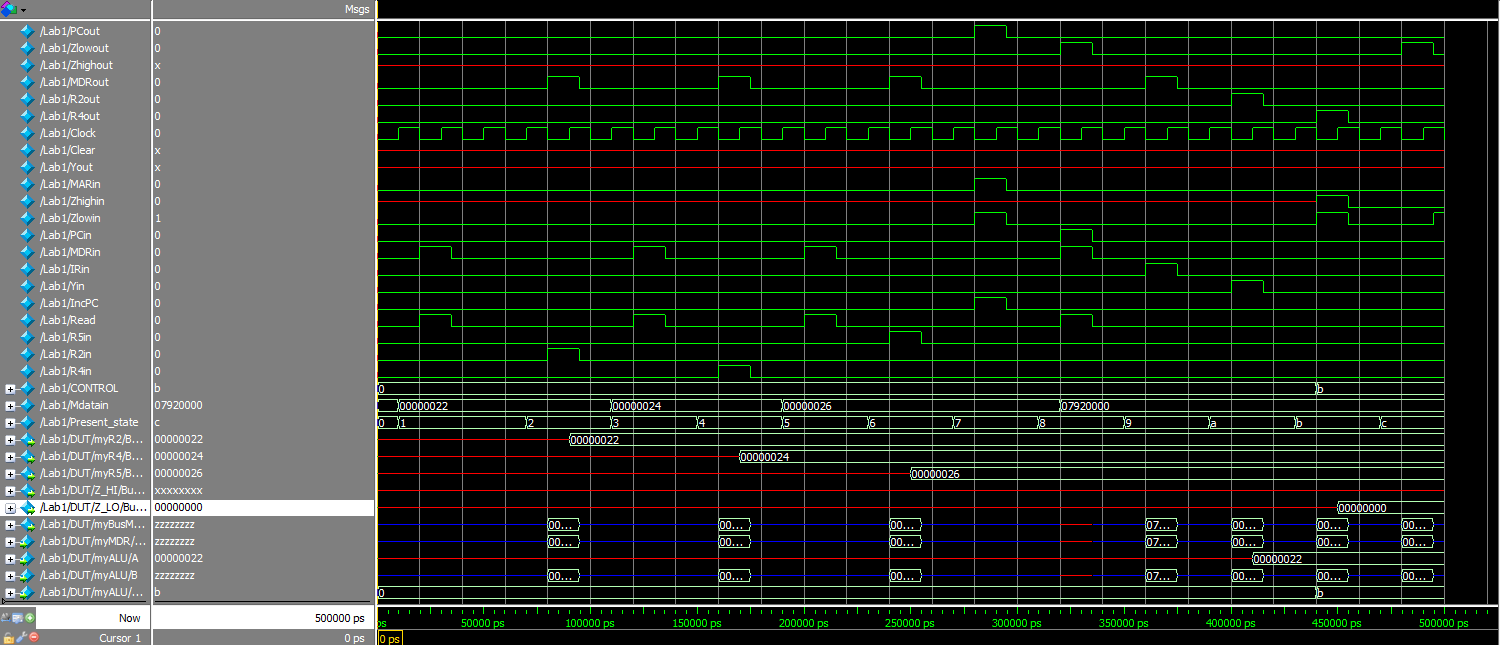
\includegraphics[width=15cm]{DIV_final_image.png}
            \caption{A screenshot of the simulated waveforms for the div R5, R2, R4 instruction, without remainder.}
        \end{center}
    \end{figure}

    \subsection{shr R5, R2, R4}
    This instruction demonstrates the ALU's shift right circuitry. This differs from the control sequence in the testbench shown with the removal of a second input. That is, R4 is no longer used. Furthermore, the CONTROL signal is changed to that of the right shift command. The control sequence for this instruction can be found below in Appendix \ref{SHR}.
    
    \begin{figure}[h!]
        \begin{center}
            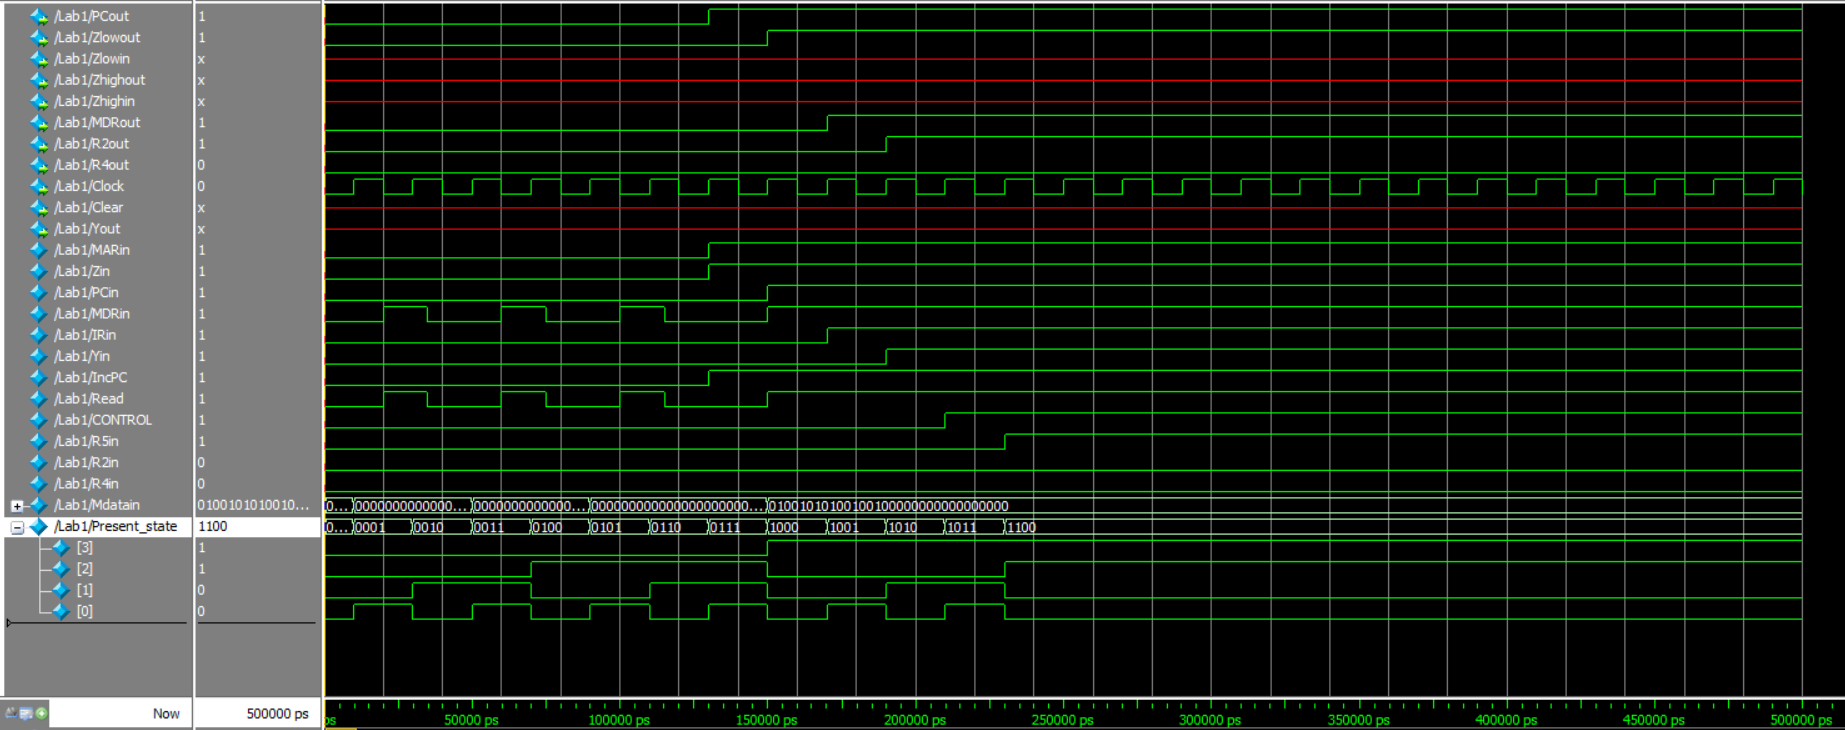
\includegraphics[width=15cm]{shr}
            \caption{A screenshot of the simulated waveforms for the shr R5, R2, R4 instruction}
        \end{center}
    \end{figure}

    \subsection{shl R5, R2, R4}
    This instruction demonstrates the ALU's shift left circuitry. Its control sequence is identical to that of the shift right command with the exception of the CONTROL signal being changed to that of the shift left instruction. The control sequence for this instruction can be found below in Appendix \ref{SHL}.

    \begin{figure}[h!]
        \begin{center}
            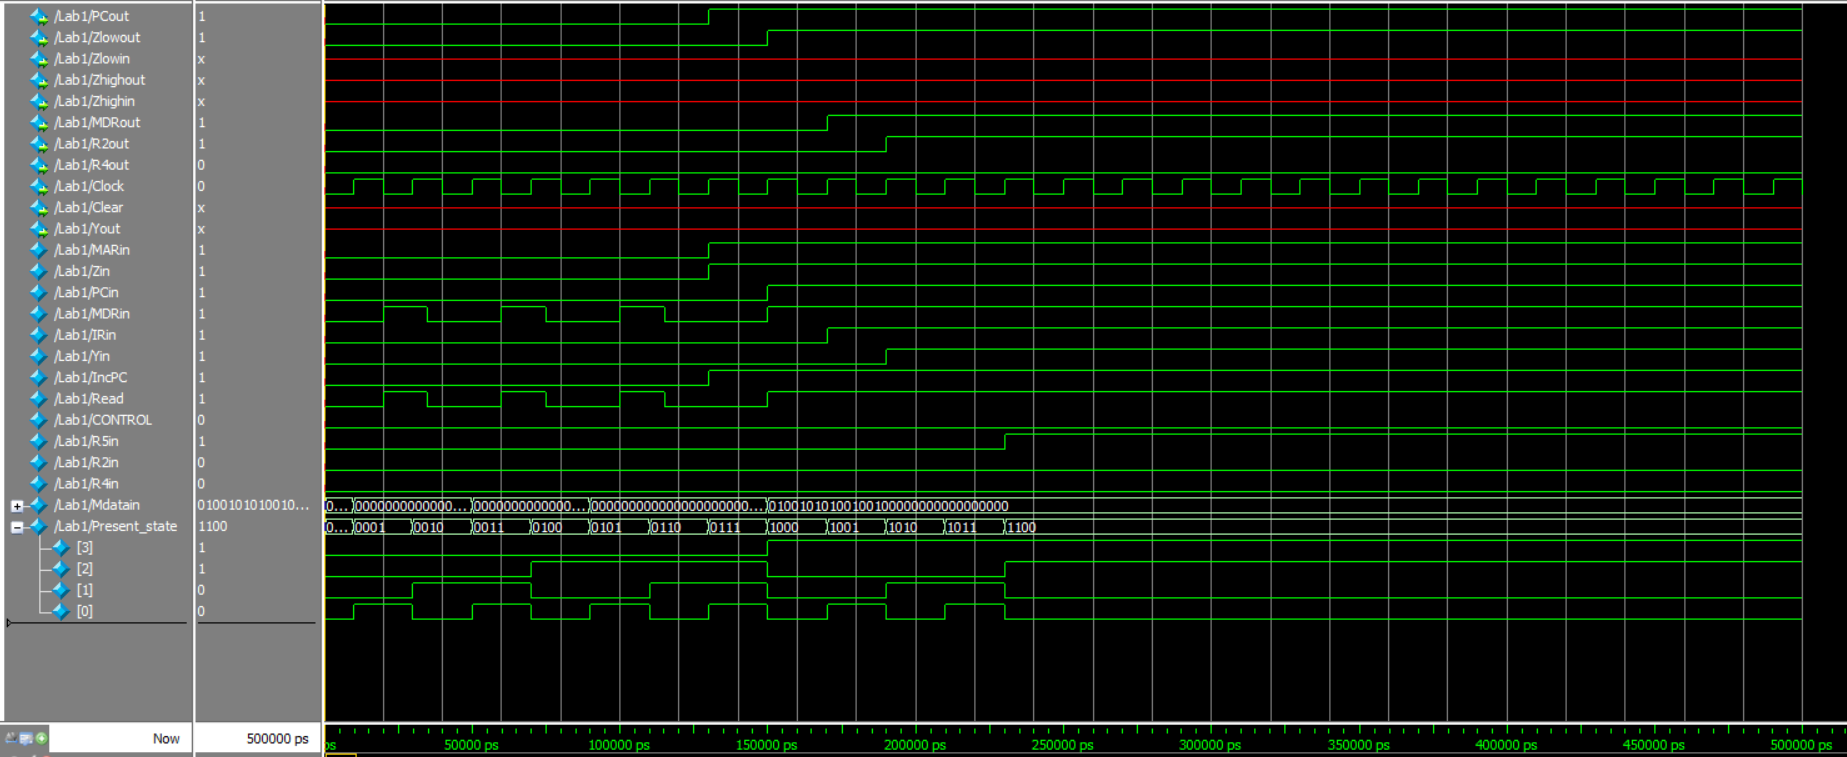
\includegraphics[width=15cm]{shl}
            \caption{A screenshot of the simulated waveforms for the shl R5, R2, R4 instruction}
        \end{center}
    \end{figure}

    \subsection{ror R5, R2, R4}
    This instruction demonstrates the ALU's rotate right circuitry. Its control sequence is identical to that of the shift right command with the exception of the CONTROL signal being changed to that of the rotate right instruction. The control sequence for this instruction can be found below in Appendix \ref{ROR}.

    \begin{figure}[h!]
        \begin{center}
            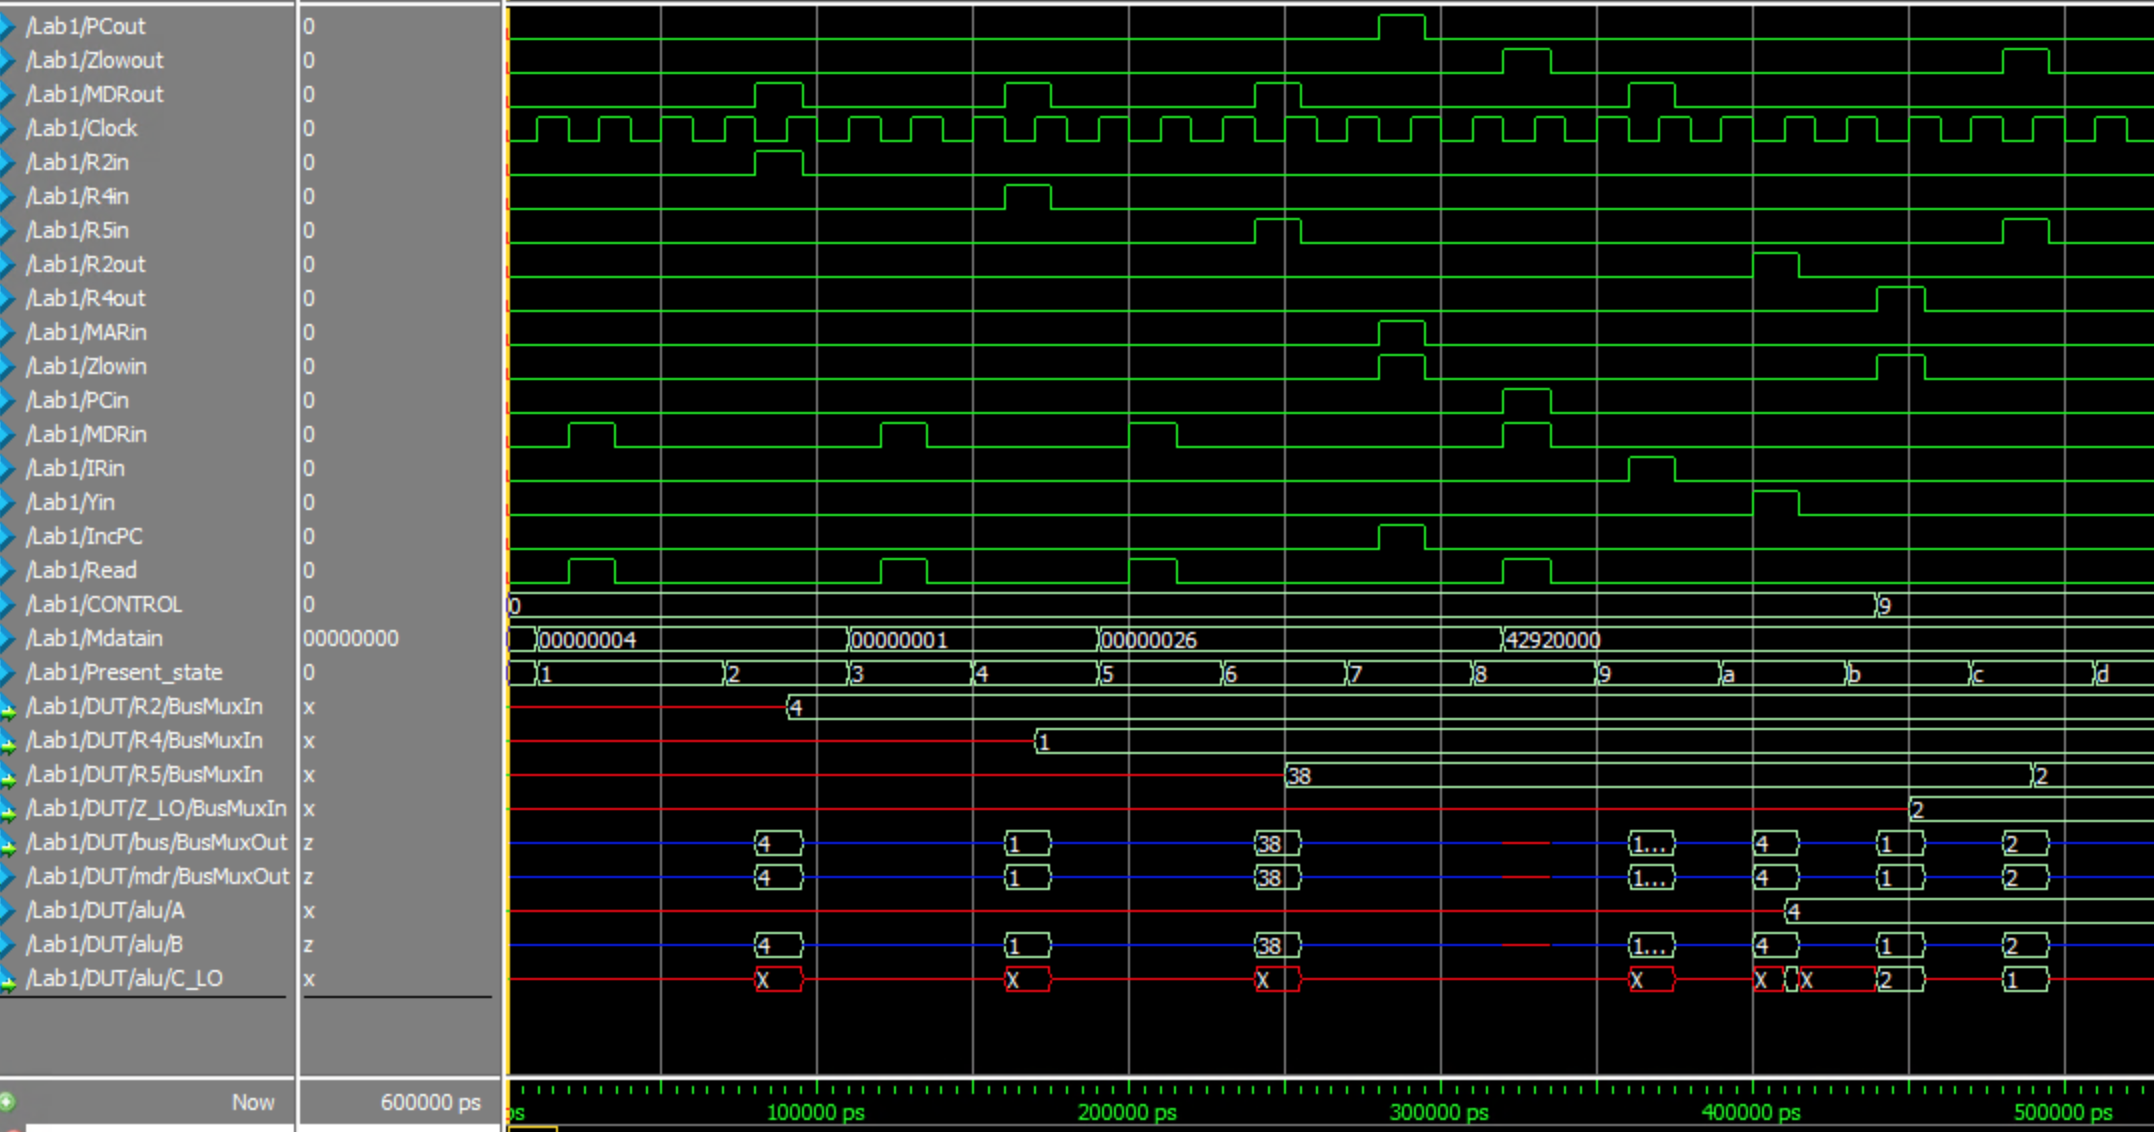
\includegraphics[width=15cm]{ROR_FINAL.png}
            \caption{A screenshot of the simulated waveforms for the ror R5, R2, R4 instruction}
        \end{center}
    \end{figure}

    \subsection{rol R5, R2, R4}
    This instruction demonstrates the ALU's rotate left circuitry. Its control sequence is identical to that of the shift right command with the exception of the CONTROL signal being changed to that of the rotate left instruction. The control sequence for this instruction can be found below in Appendix \ref{ROL}.

    \begin{figure}[h!]
        \begin{center}
            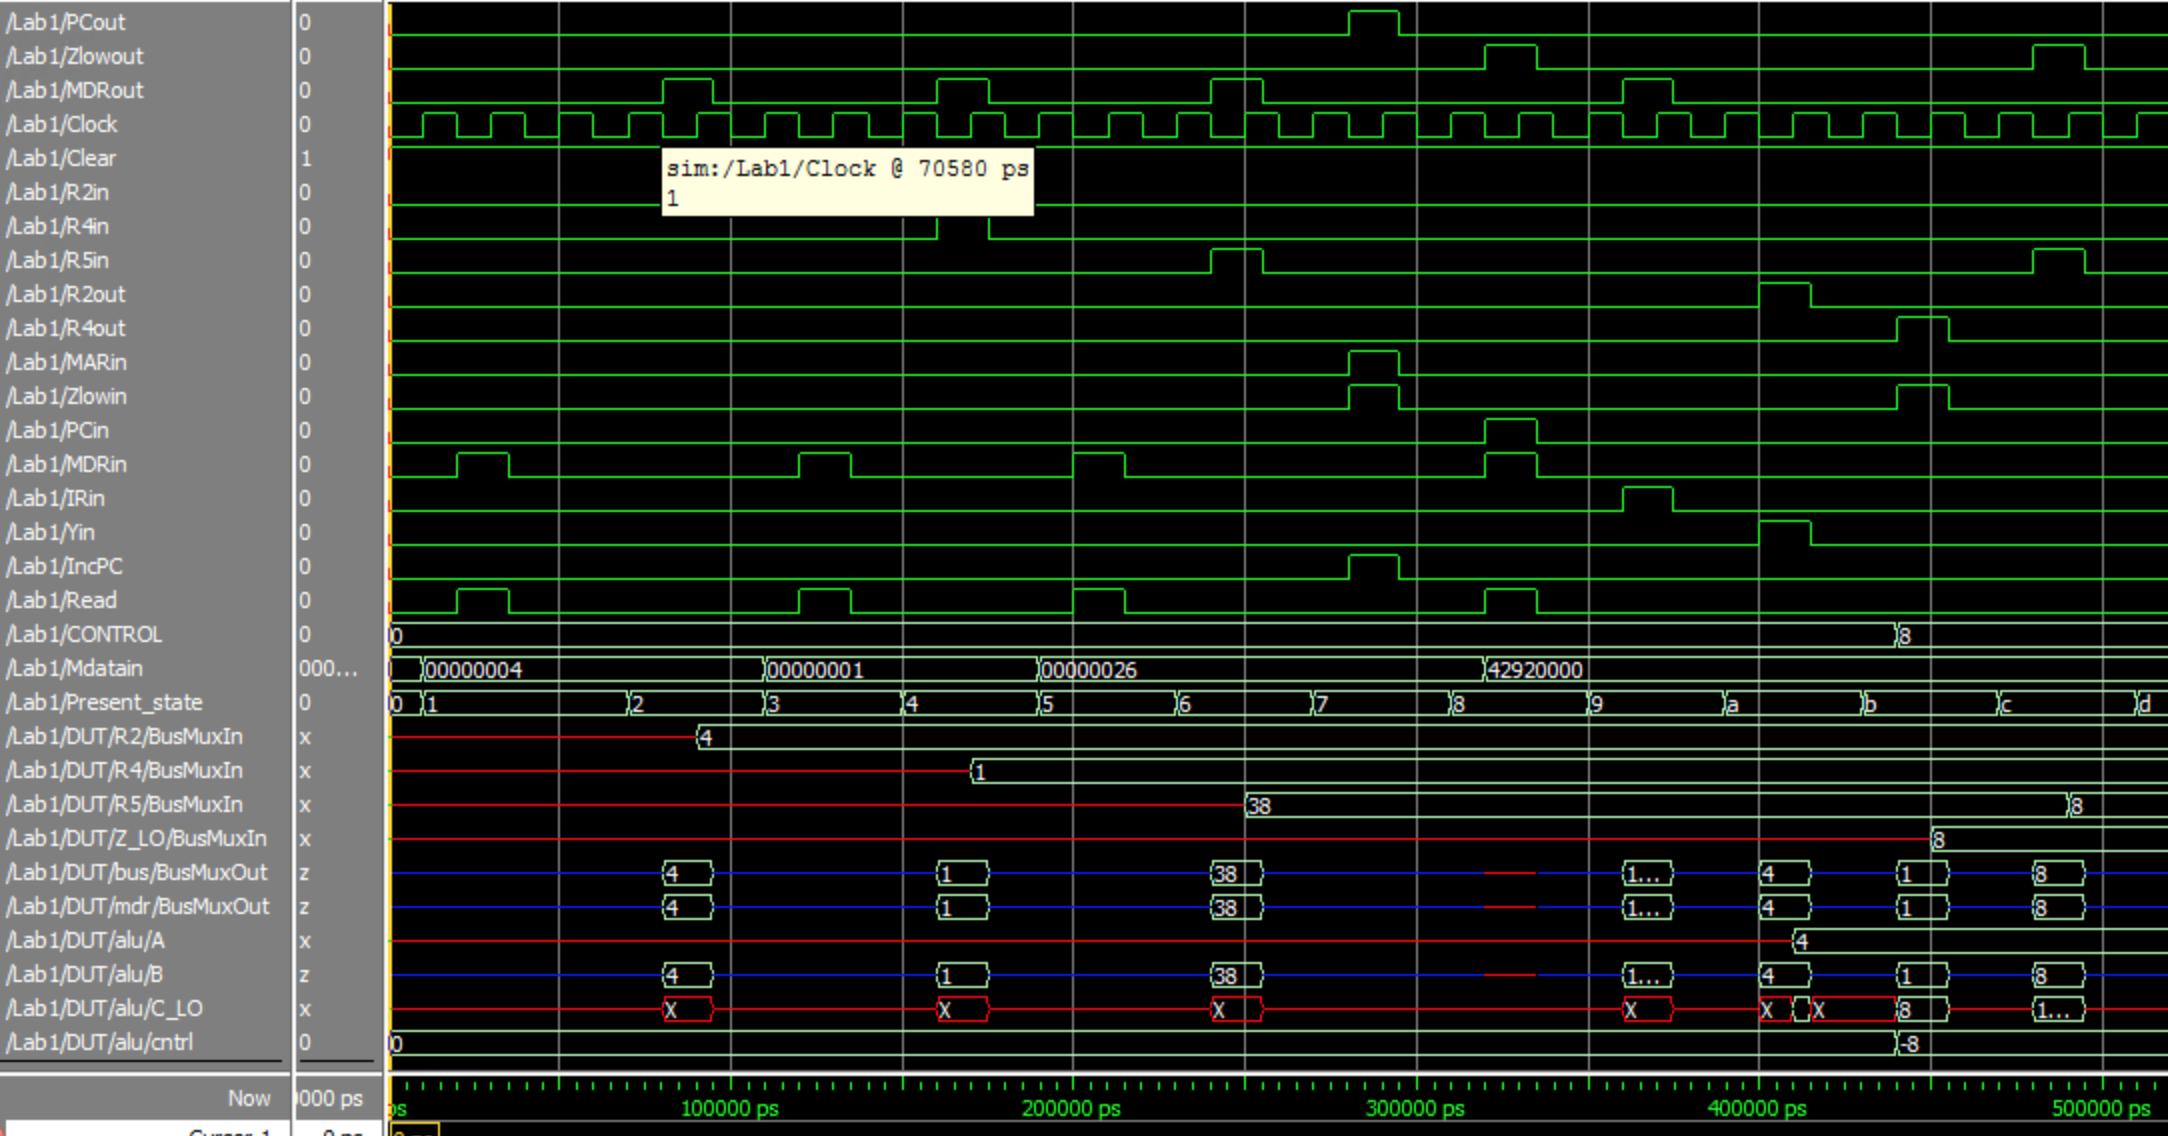
\includegraphics[width=15cm]{ROL_FINAL.png}
            \caption{A screenshot of the simulated waveforms for the rol R5, R2, R4 instruction}
        \end{center}
    \end{figure}

    \subsection{neg R5, R2}
    This instruction demonstrates the ALU's negation circuitry. The control sequence only has 4 stages. States 0-2 are identical and the changes can be found in states 3 and 4. Also, no second input is required. The CONTROL signal is changed to that of the negate instruction. The control sequence for this instruction can be found below in Appendix \ref{NEG}.

    \begin{figure}[h!]
        \begin{center}
            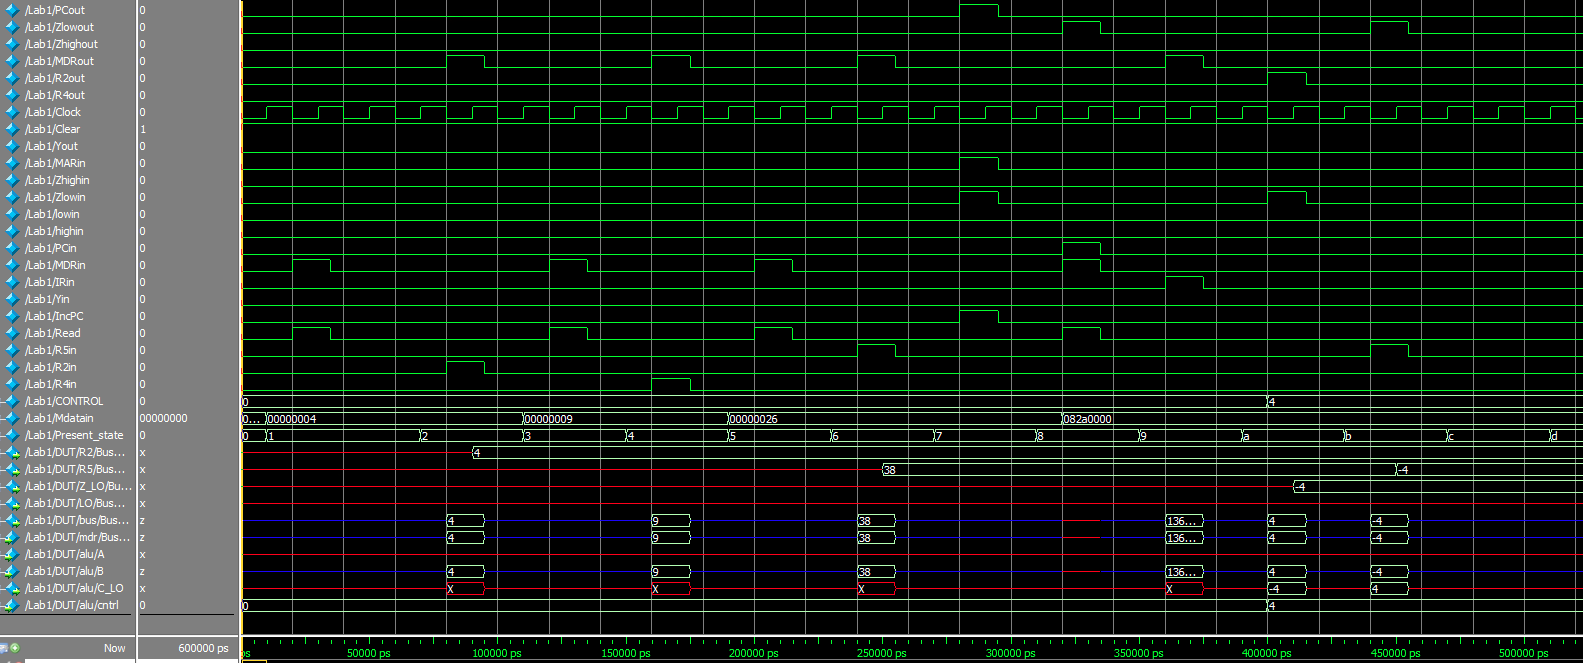
\includegraphics[width=15cm]{NEG_FINAL.png}
            \caption{A screenshot of the simulated waveforms for the neg R5, R2 instruction}
        \end{center}
    \end{figure}

    \subsection{not R5, R2}
    This instruction demonstrates the ALU's not circuitry. Its control sequence is identical to that of the negation instruction with the exception of the CONTROL signal being changed to that of the negation instruction. The control sequence for this instruction can be found below in Appendix \ref{NOT}.
    \begin{figure}[h!]
        \begin{center}
            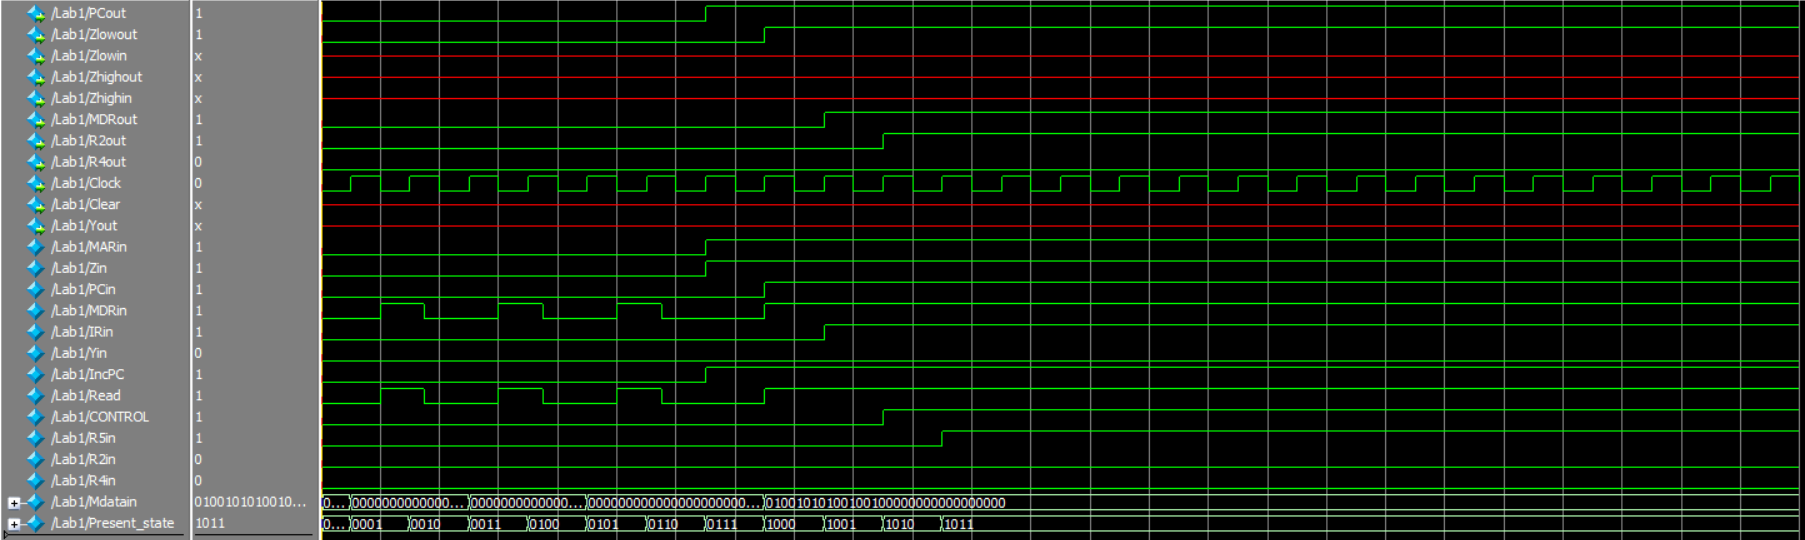
\includegraphics[width=15cm]{not}
            \caption{A screenshot of the simulated waveforms for the not R5, R2 instruction}
        \end{center}
    \end{figure}

\appendix
\section{Testbench} \label{Testbench}
    \lstinputlisting{Lab1.v}
\section{Bus} \label{Bus}
    \lstinputlisting{Bus.v}
\section{MDR}\label{MDR}
    \lstinputlisting{MDR.v}
\section{Datapath} \label{Datapath}
    \lstinputlisting{datapath.v}
\section{ALU} \label{ALU}
    \subsection{ALU}
        \lstinputlisting{ALU.v}
    \subsection{And}
        \begin{lstlisting}
        0   :   C = A & B;
        \end{lstlisting}
    \subsection{Or}
        \begin{lstlisting}
		1   :   C = A | B;
        \end{lstlisting}
    \subsection{Add}
        \begin{lstlisting}
        2   :   C = A + B;
        \end{lstlisting}
    \subsection{Subtract}
        \begin{lstlisting}
		3   :   C = A - B;
        \end{lstlisting}
    \subsection{Multiplication}
        \lstinputlisting{ArithmeticLogic/div.v}\label{MUL_ALG}
    \subsection{Division}
        \lstinputlisting{ArithmeticLogic/div.v}\label{DIV_ALG}
    \subsection{Negation}
        \begin{lstlisting}
        4   :   C = -B; //negation function
        \end{lstlisting}
    \subsection{Not}
        \begin{lstlisting}
        5   :   C = !B; // logical not 
        \end{lstlisting}
    \subsection{Shift Left}
        \begin{lstlisting}
        6   :   C = A <<< B; // left arithmetic shift - A = how many shifts, B = the number you want to shift 
        \end{lstlisting}
    \subsection{Shift Right}
        \begin{lstlisting}
        7   :   C = A >>> B; // right arithmetic shift - A = how many shifts, B = the number you want to shift 
        \end{lstlisting}
    \subsection{Rotate Left}
        \lstinputlisting[firstline=25,lastline=28]{ALU.v}
    \subsection{Rotate Right}
        \lstinputlisting[linerange=21-24]{ALU.v}
\section{Control Sequences}
    \subsection{and R5, R2, R4} \label{AND}
        \lstinputlisting{TestBenches/tb_AND.v}
    \subsection{or R5, R2, R4} \label{OR}
        \lstinputlisting{TestBenches/tb_OR.v}
    \subsection{add R5, R2, R4} \label{ADD}
        \lstinputlisting{TestBenches/tb_ADD.v}
    \subsection{sub R5, R2, R4} \label{SUB}
        \lstinputlisting{TestBenches/tb_SUB.v}
    \subsection{mul R2, R4} \label{MUL}
        \lstinputlisting{TestBenches/tb_MUL.v}
    \subsection{div R2, R4} \label{DIV}
        \lstinputlisting{TestBenches/tb_DIV.v}
    \subsection{shr R5, R2, R4} \label{SHR}
        \lstinputlisting{TestBenches/tb_SHR.v}
    \subsection{shl R5, R2, R4} \label{SHL}
        \lstinputlisting{TestBenches/tb_SHL.v}
    \subsection{ror R5, R2, R4} \label{ROR}
        \lstinputlisting{TestBenches/tb_ROR.v}
    \subsection{rol R5, R2, R4} \label{ROL}
        \lstinputlisting{TestBenches/tb_ROL.v}
    \subsection{neg R5, R2} \label{NEG}
        \lstinputlisting{TestBenches/tb_NEG.v}
    \subsection{not R5, R2} \label{NOT}
        \lstinputlisting{TestBenches/tb_NOT.v}
\end{document}
